\chapter{System zur Visualisierung akustischer Schmerz-Scores}


Das Ziel dieser Arbeit ist die Ableitung des Schmerz-Scores aus einem Audiosignal sowie die darauf folgende Visualisierung dieser Schmerz-Scores. Folgende Anforderungen werden an das System gestellt:
\begin{enumerate}
	\item Das System muss dazu in der Lage sein, aus den akustischen Eigenschaften des Weinens die Schmerz-Score abzuleiten
	\item Das System muss dazu in der Lage sein, die Schmer-Score zu visualiseren.
	\item Die Verarbeitungspipeline muss genug Flexibilität bieten, um beliebige Pain-Scores einzubinden. 
	\item Die Analyse muss auch bei nicht-optimalen akustischen Bedingungen Einsatzfähig sein.
	\item Die Methoden müssen kontinuierlich eingesetzt werden können. Das heißt, dass zu einem Analysezeitpunkt nur Informationen verwendet werden können, die nicht in der Zukunft liegen.
\end{enumerate}

Im folgenden wird ein Überblick über bereits verföffentlichte Ansätze zur Analyse von akustischen Signalen Neugeborener oder sonstiger automatisierter Systeme zur Ableitung der Pain-Score gegeben.

\section{Literatur-Übeblick}
\label{sec:system_literature}

Bei der Aufgabenstellung handelt es sich grob betrachtet um einen Klassifikations/Regressions-Aufgabe, bei der aus den Eigenschaften des Audiossignals mit den Kindlichen Lautäußerungen eine Schluss gezogen werden soll. In dieser Aufgabenstellung ist der Schluss eine Pain-Score. An dieser Stelle wird ein Überblick über Veröffentlichungen gegeben, in denen ähnliche Aufgabenstellungen bearbeitet worden.

Der Großteil der Veröffentlichungen stellt Systeme Klassifikation einzelner Cry-Units vor, entweder bezüglich der Wein-Ursache (Hunger, Angst, Schmerz... ) oder zur Diagnose bestimmer Krankheiten. Diese Methoden sind nicht für die kontinuierliche Analyse geeignet, sondern haben das Ziel, bezüglich einer bereits vorliegenden Cry-Unit eine möglichst hohe Klassifizierungs-Accuracy zu erzielen. Probleme wie Hintergrundrauschen, Berechnungsaufwand oder kontextuelle Informationen werden selten mit in Betracht gezogen. Beispiele für solche Systeme sind die von Abdulaziz et al \cite{class_abdulaziz} oder Furh et al \cite{comparisonOfLearning}.

Várallyay stellt in seiner Dissertation \glqq Analysis of the Infant Cry with Objective Methods\grqq{} \cite{cry_thesis} Methoden zur automatisierten Analyse kindlicher Lautäußerungen vor. Das eigentliche Ziel der Dissertation ist die Erforschung der Unterschiede zwischen den Lautäußerungen gesunder und tauber Neugeborener. Die automatisierte Verarbeitungs-Pipeline der Audiosignale ist dabei ein \glqq Nebenprodukt\grqq{} zur schnelleren Auswertung der Signale. Die Auswertung muss nicht kontinuierlich erfolgen. In der vorgestellten Verarbeitungspipeline wird das Eingangssignal in Zeitfenster weniger Millisekunden zerlegt und jedes Fenster auf Basis der Fenstereigenschaften als Stimmhaft oder nicht-Stimmhaft klassifiziert. Die stimmhaften Signalfenster werden zu \emph{Segmenten} zusammengefasst (in Kapitel \ref{sec:acousticModel} als Cry-Unit bezeichnet). Auf Basis der Segmente werden Auswertungen bezüglich der Zeit-Bereiches (Durchschnittliche Segmentlänge, Pausenlängen etc.), des Frequenz-Bereiches (Grund-Frequenz, Formanten-Frequenzen etc.) und des Melodie-Verlaufes (Melodie-typ) angestellt. Analysiert wurden Signale mit einer Länge von 10 bis 100 Sekunden, die Lautäußerungen von Babies mit oder ohne Hörbehinderung beinhalten. Aus den Auswertungsergebnisse stellt Várallyay die wichtigsten Unterscheidungsmerkmale zwischen tauben und gesunden Babies fest. In der Dissertation \cite{cry_thesis} wird ein Überblick über das Vorgehen und die Ergebnisse gegeben. Die Verarbeitungsschritte werden detailllierter in einzelnen Veröffentlichungen beschrieben, auf die der Autor dieser Arbeit jedoch kein Zugriff gewährt wurde.

Cohen et al haben 2012 in dem Paper \glqq Infant Cry Analysis and Detection \grqq{} \cite{cohenCry}  ein System zur Analyse der akustischen Signale von Neugeborenen vorgestellt. Dieses System klassifziert die Audio-Signale in eine der drei Klassen \emph{Cry, No Cry} und \emph{No Activity}. Mit \emph{Cry} sind Lautäußerungen gemeint, die eine potentiell Gefahr für das Baby anzeigen, wie z.B. wie Schmerz oder Hunger. \emph{No Cry} meint, dass das Baby zwar Laute von sich gibt, diese aber keine potentielle Gefahr anzeigen. emph{No Activity} meint keinerlei Lautäußerung. Die Verarbeitungs-Pipeline wird detailliert vorgestellt und ist für die kontinuierliche Verarbeitung mit einer gewissen Verzögerungszeit spezialisiert. Das Signal wird in überlappende \emph{Segmente} \`{a} 10 Sekunden zerlegt. Die Stimmaktivität in dem Segment wird algorithmisch festgestellt. Wenn Aktivität vorliegt, wird das Segment in Sections \`{a} 1 Sekunden zerlegt und die Stimmaktivität für jede Section analysiert. Wird genügend Stimmaktivität für eine Section festgestellt, wird die Section in \emph{Frames}) \`{a} 32 Millisekunden zerlegt und Features für jedes Signalfenster errechnet. Mit Hilfe eines Predictors werden die Frames in \emph{Cry, No-Cry, No-Activity} klassifiziert, wobei Kontextuelle Informationen der umliegenden Frames mit einbezogen werden. Aus den Klassen der Frames wird auf die Klasse der Section geschlossen, und aus den Klassen der Sections auf die Klasse des 10 Sekunden langen Segments. Das System hat in Bezug auf diese Arbeit den Vorteil, dass ebenfalls die kontinuierliche Verarbeitung im Vordergrund steht. Der Nachteil an dieser Methode ist, dass die zeitliche Einheit, für die die Klassifizierung vorgenommen wird, auf unflexibel auf 10 Sekunden festgelegt ist. Daher müsste diese Verarbeitungspipeline abgewandelt werden, um Anstelle der  Ableitung der drei genannten Klassen einer Pain-Score zu verwenden, die einen längeren Beobachtungszeitraum als 10 Sekunden benötigt.

Pal et al  haben 2006 in dem Paper \glqq Emotion detection from infant facial experessions and cries\grqq{} \cite{palEmotion} ein System zur Emotions-Detektion bei Neugeborenen aus Aufnahmen des Gesichtsausdruck und akustischen Aufnahmen des Weinens vorgestellt. Die zu erkennenden Emotionen sind \emph{Traurigkeit, Wut, Hunger, Angst und Schmerz}. Es wird nicht erwähnt, ob die Analyse kontinuierlich oder nicht-kontinuierlich erfolgt. Bei der Verarbeitung der akustischen Signale werden die Features \emph{Grund-Tonhöhe} und die \emph{Frequenz der ersten drei Formanten} extrahiert und mit einem Klassifikations-Algorithmus klassifiziert. Es werden keinerlei Details genannt, inwiefern die Features aus kurzen Signalfenstern oder längeren Signalabschnitten errechnet werden, welche Vorverarbeitungsschritte angewandt werden und ob die Klassfizierung auf Ebene der Signalfenster oder über längere Zeitabschnitte hingweg geschieht. Die Veröffentlichung liefert Ideen über mögliche Features, bietet jedoch keinen Einblick in die Verarbeitungspipeline.

Zamzi et al  haben 2016 in dem Paper \glqq An Approach for Automated Multimodal Analysis of Infants' Pain\grqq{} \cite{zamziMultimodal} ein System zur automatisierten und kontinuierlichen mutlimodalen Analyse von Neugeborenen zur Ableitung des Schmerzes vorgestellt. Das System trägt den Namen \emph{MPAS}. Der Insgesamte Schmerzgrad wird aus den Analyseergebnissen der monomdaler Schmerzindikatoren für \emph{Gesichtsausdruck, Körperbewegung, Vitalfunktionen und Weinen} errechnet. Das Ziel des Projektes kommt der Aufgabenstellung dieser Masterarbeit am nächsten, da es auch um die Ableitung von Schmerz in einem mulitmodalen Verbund geht. Es wird jedoch nicht die Anfoderung gestellt, Flexibilität in der Wahl der Pain-score zu bieten. Während in der Veröffentlichung die Analyse der ersten drei genannten Schmerzindikatoren angekündigt wird, werden daraufhin die Methoden zur Analyse der akustischen Signale \emph{nicht} weiter erläutert. Auch die ersten Validierungs-Ergebnisse beziehen sich nur auf den Gesichtsausdruck, Körperbewegung und Vitalfunktionen. Es ist nicht klar, ob die Miteinbeziehung akutischer Signale fallen gelassen wurde, oder in Zukunft mit einbezogen werden wird. Die Ausführungen konzentrieren sich dazu vermehrt auf die Methoden zur Kombination der Auswertungsergebnisse der monomodalen Schmerzindikatoren. Die Verarbeitungs-Pipelines der monomdalen Schmerzindikatorn werden nur grob vorgestellt.

\section{Verarbeitungs-Pipeline}

In Kapitel \ref{sec:system_literature} wurden verschiedene Systeme vorgestellt, deren Problemstellungen dem Thema dieser Masterarbeit ähneln. Keine der präsentierten Verarbeitungs-pipelinen eignet sich, um mit nur leichten Anpassungen übernommen werden zu können: Entweder sind die Verarbeitungsschritte nicht für die kontinuierliche Verarbeitung konzipiert \cite{class_abdulaziz} \cite{comparisonOfLearning} \cite{cry_thesis}, nicht genügen abstrahiert, um für andere Klassifizierungen als die ursprünglich geplanten abgewandelt werden zu können \cite{cohenCry}, oder stellen die Verarbeitungs-pipeline nicht vor \cite{palEmotion} \cite{zamziMultimodal}.



Das Ziel dieser Arbeit ist die Ableitung des Schmerz-Scores aus einem Audiosignal sowie die darauf folgende Visualisierung dieser Schmerz-Scores. Um diese komplexe Aufgabenstellung zu lösen, wird sie in einzelne Arbeitspakete zerlegt. Welche Arbeitspakete formuliert werden, ist davon abhängig, aus welcher Perspektive die Aufgabenstellung grundlegend betrachtet wird. So kann sie beispielsweise als Unterproblem der Schrei-Forschung betrachtet werden, woraufhin sie mit Hilfe des in Kapitel \ref{sec:acousticModel} vorgestellten Vokabulars modelliert wird. Ebenso kann die Aufgabe grundlegend als Problem der automatisierten Spracherkennung verstanden werden, woraufhin ein in diesem Wissenschaftsgebiet üblicher Verarbeitungsprozess entworfen werden würde. Dieser Ansatz wurde beispielsweise in dem von Cohen et al vorgestellten System zur Kategorisierung von Audioaufnahmen von Babys in (0) Nicht-Weinen und (1) Weinen gewählt.\cite{automaticCryDetection} 

In dieser Arbeit wurde sich für den Ansatz entschieden, die Arbeitspakete aus Sicht der Schreiforschung zu modellieren und dabei das in \ref{sec:acousticModel} vorgestellte Vokabular zu verwenden. Die einzelnen Arbeitspakete werden daraufhin mit Methoden der Signalverarbeitung gelöst. Hintergrund ist, dass die Arbeitsweise des Systems in Zukunft einfacher Medizinern vermittelbar ist, da die verwendeten Begrifflichkeiten leichter zugänglich sind. Das folgende Vorgehen wird dazu vorgeschlagen:

\begin{enumerate}[leftmargin=*]
	\item Kontinuierliche Betrachtung des Eingangssignals
	\item Markierung der Cry-Units / Expirations in diesem Einganssignal (und eventuelle Kategorisierung in Phonation, Hyper-Phonation und Dysphonation)
	\item Gruppierung der markierten Cry-Units zu Cry-Segments
	\item Errechnung der charakteristischen Eigenschaften der Segmente
	\item Ableitung der Pain-Score aus den Eigenschaften der Segmente.
	\item Visualisierung dieser Pain-Score.
\end{enumerate}

\begin{figure}[H]
	\centering
	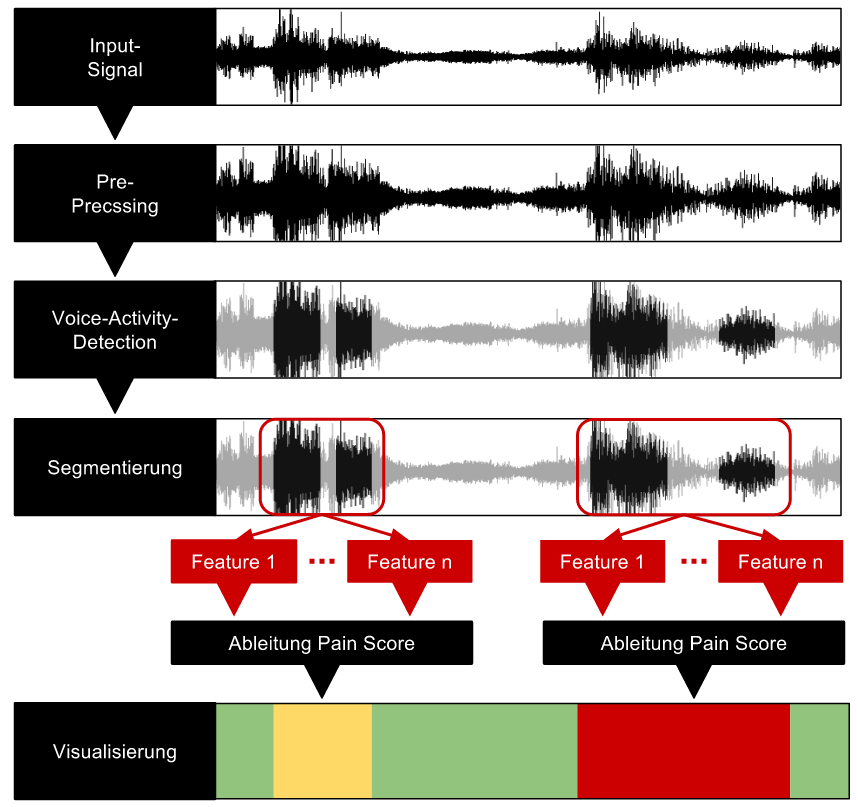
\includegraphics[width=0.75\textwidth]{bilder/architektur.png}
	\caption{Architektur des Systems}
	\label{img:architecture-overview}
\end{figure}

Diese Arbeitspakete werden nun auf Probleme der automatisierten Spracherkennung abgebildet. Abbildung \ref{img:architecture-overview} veranschaulicht die Architektur, die sich daraus ergibt. Eingang in das System ist das Audiosignal, welches kontinuierlich in das System gegeben wird. Das Signal passiert daraufhin die folgenden Verarbeitungsschritte:

\begin{enumerate}[leftmargin=*]
	\item \textbf{Pre-Processing}. Das Signal wird vorverarbeitet. Durch die Anwendung von Filtern (linearen wie nicht-linearen) werden die darauf folgenden Verarbeitungsschritte vereinfacht. Das Ergebnis ist ein vorverareitetes Signal. Dieser Verarbeitungsschritt wurde zu den Zeiten der manuellen Schrei-Analyse noch nicht mit einbezogen, ist jedoch in der automatisierten Spracherkennung üblich.
	\item \textbf{Voice-Activity-Detection}. In dem Signal müssen diejenigen Stellen erkannt werden, die die Stimme des Babys enthalten. Dazu wird das Signal in kurze Fenster weniger Millisekunden Länge zerlegt und jedes Fenster als \emph{Stille} (0) oder \emph{Stimme} (1) markiert. Zusammehängende, als stimmhaft erkannte Signalfenster werden daraufhin zu \emph{Cry-Units} gruppiert.
	\item \textbf{Segmentierung}, das heißt die Gruppierung der markierten Cry-Units zu \emph{Cry-Segments}.
	\item \textbf{Feature-Extraction}, das heißt die Berechnung von Eigenschaften für jedes Segment, die für die Ableitung der Pain-Scores von Interesse sind, wie beispielsweise die Duration. Die errechneten Features müssen sich dabei nicht auf diejenigen beschränken, die von H Golub und M Corwin \cite{cryModel} vorgestellt wurden, da diese zur (vermeintlichen) Unterscheidung der Wein-Ursache, und nicht zur Ableitung einer Pain Score gedacht waren.
	\item \textbf{Ableitung der Pain Score} aus den errechneten Eigenschaften.
	\item \textbf{Visualisierung} der errechneten Pain-Score.
\end{enumerate}

Für jedes dieser Module werden verschiedene Lösungsansätze vorgestellt und zumindest ein Lösungsansatz implementiert. Das Pre-Processing wird in Kapitel \ref{sec:preprocessing} vorgestellt, die Voice-Activity-Detection in Kapitel \ref{sec:vad}, die Segmentierung in Kapitel ........

\section{Preprocessing}
\label{sec:preprocessing}

Beim Preprocessing wird das Signal so vorverarbeitet, dass Störeinflüsse auf die darauf folgenden Verarbeitungsschritte von vorneherein minimiert werden. Welches Pre-Processing durchgefüht wird, ist Abhägig von der konrketen Aufgabenstellung. So werden beispielsweise bei einigen Algorithmen zur Voice-Activity-Detection, also dem markieren stimmhafter Signalabschnitte, Tiefpass, Hochpass- und Bandpassfilter eingesetzt, um diejenigen Frequenzanteile herauszufiltern, die von der Stimme nicht produziert werden können \cite{vad_entropy} \cite{vad_ceps} \cite{vad_kola}. Bei einigen Pitch-Detection-Algorithmen wird \emph{Centerclipping} eingesetzt, also das 0-Setzen von Samples mit $ x[i] < 0.5 \cdot $ Maximalaussteuerung.\cite{czechPitch} 

In dieser Arbeit wurde sich für eine Vorverarbeitung entschieden, bei der das Signal hinsichtlich seiner Dynamik im Zeitbereich eingegrenzt wird. Dies ist ein typischer Vorverarbeitungschritt bei Sprachaufnahmen. Hintergrund ist, dass sehr kurz, aber sehr laute Pegelspitzen weit über dem Durchschnittspegel des Gesamtsignals den Maximalwert des Signals unnötig begrenzen und die Signalenergie so gering halten. Da die Testsignale, die in dieser Arbeit verwendet werden, aus inhomgenen Quellen stammen und sehr unterschiedliche Lautstärken haben, wird so gewährleistet, dass sie zumindest ähnliche Energien haben. An dieser Stelle werden (noch) keine Frequenanteile herausgefiltert, um keine Frequenzen zu verlieren, die in den späteren Verareitungsschritten wieder Voice-Activity-Detection \ref{sec:vad} oder der Feature-Extraction eventuell noch benötigt werden.

Die Dynamikeinschränkung wird mit Hilfe eines Audiokompressor umgesetzt. Ein Audiokompressor verringert Signalspitzen, die über einen festgelegten \emph{Schwellwert (Threshold)} liegen, um ein festgelegtes \emph{Verhältnis (Ratio)}. Ein Threshold von 0.3 mit Ratio von 0.5 bedeutet beispielsweise, dass alle Signalspitzen, die den Wert 0.3 überschreiten oder -0.3 unterschreiten, um 50\% verringert werden. Ein Kompressor kann auf die Überschreitung des Thresholds erst nach einer als \emph{Attack} bezeichneten Verzögerung reagieren, und bei erneuten Verlassen des Thresholdes mit einer als \emph{Release} bezeichneten Verzögerung nachwirken. Signalspitzen werden so verringert und die Lautstärke-Dynammik eingeschränkt. Die tatsächliche Erhöhung der Signalenergie geschieht im Anschluss durch die Anhebung der insgesamten Signallautstärke, wie Beispielsweise der Normalisierung des Signals auf den Maximalpegel. Abbildung \ref{img:compressor} zeigt die Parameter eines solchen Audio-Kompressors.

\begin{figure}[h]
	\centering
	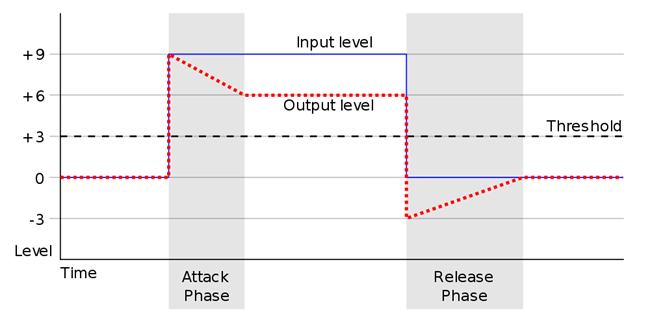
\includegraphics[width=0.6\textwidth]{bilder/compressor.png}
	\caption{Parameter eines Audio-Kompressors}
	\label{img:compressor}
\end{figure}

Der entwickelte Kompressor automatisiert die Einstellung von Threshold und Ratio auf Grundlage des Root-Mean-Square (RMS) des Signales $x$ der Länge $N$. Der RMS-Wert ist ein Maß für die durchschnittliche Signalenergie und wird wie nach Formel \ref{eq:rms} berechnet. Threshold und Ratio werden nach den Formeln \ref{eq:THold} und \ref{eq:ratio} berechnet, wobei der Parameter $r_a$ den Ziel-RMS-Wert anbgibt und mit dem Wert.

\begin{equation}
\text{RMS}(x) = \sqrt{\frac{1}{N}\sum_{n=0}^{N-1}x[n]^2}
\label{eq:rms}
\end{equation}
\begin{equation}
\text{THold}(x) = \bigg[\frac{\text{RMS}(x[])}{r_a}\bigg]^{2}
\label{eq:THold}
\end{equation}
\begin{equation}
\text{Ratio}(x) = \bigg[\frac{\text{RMS}(x[])}{r_a}\bigg]^{2}
\label{eq:ratio}
\end{equation}

Abbildung \ref{img:compressing01} zeigt das ein Signal vor und nach dem Preprocessings. Zu sehen ist, dass die Lautstärke der einzelnen Schrei-Einheiten nach der Anpassung einheitlicher ist. 

\begin{figure}[h]
	\centering
	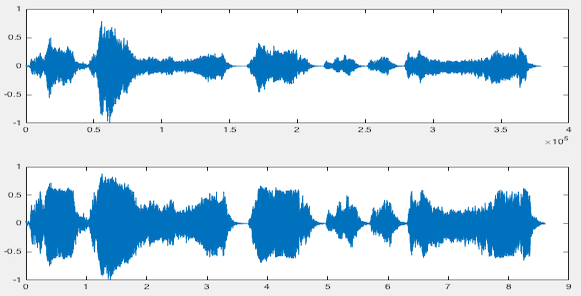
\includegraphics[width=0.6\textwidth]{bilder/compressing01.png}
	\caption{Ergebnis des Preprocessings}
	\label{img:compressing01}
\end{figure}

\section{Voice Activity Detection}
\label{sec:vad}

Das Ziel ist, in einem Audiosignal diejenigen Stellen zu markieren, in denen Schreigeräusche vorliegen. Abbilung \ref{img:vad01} visualisiert ein Beispiel für eine solche Markierung: Zu sehen ist der Zeitbereich eines Audiosignales mit drei klar erkennbaren Cry-Units. Die Rote Linie, die das Signal überspannt, bildet die Zeiteinheiten des Eingangssignales in die binären Kategorien \emph{Stimmhaft} und \emph{Stille} ab.

\begin{figure}
	\centering
	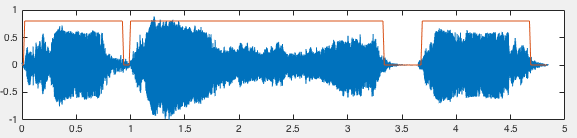
\includegraphics[width=0.6\textwidth]{bilder/VAD_01.png}
	\caption{Markierung von Schreigeräuschen im Audiosignal}
	\label{img:vad01}
\end{figure}

Das zu lösende Probem wird als \emph{Voice Activity Detection (VAD)} oder auch \emph{Speech Detection} bezeichnet. Das Ziel ist die Unterscheidung von denjenigen Zeiträumen im Signal, in denen Stimme enthalten ist, von denen, in denen keine Stimme enthalten ist. Zeiträume ohne Stimme werden von nun als \glqq Stille\grqq{}, und Zeiträume mit Stimme als \glqq Stimmhaft\grqq{} bezeichnet. Die größte Herausforderung ist für VAD-Systeme die robuste Erkennung bei Signalen mit Rauschen unbekannter Stärke und Natur.\cite{vad_granada}

Der Grundlegende Aufbau eines VAD-Algorithmus ist wie folgt:
\begin{enumerate}
	\item \textbf{Windowing}: Unterteilung des Signals in (einander überlappende) Fenster, typischerweise zweistellingen Millisekunden-Bereich.
	\item \textbf{Featureextraction} aus den einzelnen Fenstern
	\item \textbf{Thresholding / Entscheidung} über Präsens oder Nicht-Präsens von Stimme für jedes Zeitfenster auf Grundlage der Features mit Hilfe von Entscheidungsregeln wie Grenzwerten.
	\item \textbf{Decision-Smoothing}, das nachträgliche Hinzufügen oder Entfernen von Entscheidungen mit Hilfe von kontextuellen Informationen der umliegenden Entschiedungen.\cite{vad_granada}
\end{enumerate}

Der an dieser Stelle entwickelte Ansatz ist eine Kombination aus den Ideen, die in \cite{vad_Easy}, \cite{vad_Lisboa}, \cite{vad_entropy}, \cite{vad_ceps} und \cite{vad_entropie02} vorgestellt wurden. 

\subsection{Windowing}
\label{sec:windowing}

Das Signal $x$ wird in Fenster $x_1...x_n$ unterteilt. Dieser Process wird als \glqq Windowing\grqq{} bezeichnet. Es wurde sich für die in \cite{vad_entropy} vorgestellte Fensterlänge von \SI{25}{\milli\second} entschieden, als Kompromiss zwischen den in \cite{vad_Easy} empfohlenen \SI{10}{\milli\second} und den in \cite{vad_ceps} empfohlenen \SI{40}{\milli\second} Die einzelnen Fenster überlappen einander um 50\%, das heisst \SI{12.5}{\milli\second}.

\subsection{Feature Extraction}
\label{sec:featExtraction}


Für jedes Signalfenster $x_1...x_n$ à \SI{25}{\milli\second} werden die folgenden Features aus den Kategorien \textbf{Zeitbereich}, \textbf{Frequenzbereich}, \textbf{Cesptrum} und \textbf{Autokorrelation} berechnet.

\subsubsection{Zeit-Bereich}
\label{sec:timeFeats}

Im \textbf{Zeit-Bereich} werden die beiden Features \emph{Root-Mean-Square}-Wert $[RMS]$ und \emph{Zero-Crossing-Rate} $[ZCR]$ berechnet. 

In \cite{vad_Easy} wird die Energy eines Zeitfensters für die Voice Activity Detection berechnet. Um den errechneten Wert besser ins Verhältnis zum Signalpegel setzen zu können, wird anstelle der Energie der RMS-Wert nach Formel \ref{eq:rms} verwendet. Ein höherer RMS-Wert weist auf das Vorhandensein von Stimme im Signalfenster hin, da diese typischerweise eine höhere Energie als das Hintergrundrauschen hat. Als zweites Feature des Zeitbereiches wird die in \cite{vad_ceps} verwendete \emph{Zero-Crossing-Rate} (ZCR) berechnet. Dabei wird der relative Anteil an Vorzeichenwechseln des Signalfensters $x_i$ nach Formel \ref{eq:zcr} berechnet. Eine höhere ZCR weist auf Stille hin, da Rauschen typischerweise einen höheren ZCR hat als periodische Signale mit tieferer Grundfrequenz. 

\begin{equation}
\text{ZCR}(x_i[]) = \sum_{1}^{N-1}|\text{sng}(x_i[n])-\text{sng}(x_i[n-1])|
\label{eq:zcr}
\end{equation}

Abbildung \ref{img:VAD_TDsignals} visualisiert ein Beispielsignal mit Babygeschrei mit einem Hintergrundrauschen mit einem Signal/Rausch-Abstand von 25 \SI{25}{\decibel}. Bei dem Signal wurden die stimmhaften Segmente magenta markiert. Für jedes Signalfenster wurden der RMS-Wert und der ZCR-Wert berechnet und als Signale mit im Graphen dargestellt, in dem für den Anfangszeitpunkt eines Zeitfenster der jeweilige berechnete Feature-Wert abgetragen wird. Die beiden Signale wurden so skaliert, dass ihr Maximalwert 1 nicht überschreitet, um ihr Verhalten bezüglich des Vorhandenseins von Stimme klarer erkennbar zu machen.

\begin{figure}[h]
	\centering
	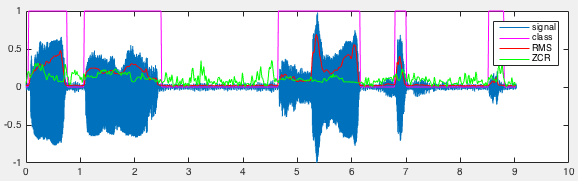
\includegraphics[width=0.6\textwidth]{bilder/VAD_TDsignals.png}
	\caption{Features des Zeitbereiches}
	\label{img:VAD_TDsignals}
\end{figure}


\subsubsection{Frequenz-Bereich}

Aus dem \textbf{Frequenz-Bereich} werden die drei Features \emph{unnormalisierte spektrale Entropie} $[SEnt_{u}]$, \emph{normalisierte spektrale Entropie}  $[SEnt_{n}]$ und \emph{dominanteste frequenzkomponenten} $[f_{Dom}]$ berechnet. 

Als Vorbereitungsschritt wurde die \emph{Kurzzeit-Fourier-Transformation} (engl. \emph{Short-Time-Fourier-Transform} STFT) nach dem Algorithmus von \cite{juliusSmith} implementiert. So wird jedes Signalfenster $x_i$ mit einem \SI{25}{\milli\second}-Hamming-Window multipliziert und daraufhin mit einer 2048-Punkte langen \emph{schnellen Fouriertransformation} (FFT) in den Frequenzbereich $F\{x_i\}$ transformiert. Weiterhin wurde für jedes Frequenz-Fenster des Magnitudensignal $X_i = |F\{x_i\}|$ berechnet und das Phasensignal jedes Zeitfensters verworfen, da für keines der Features Phaseninformationen von Interesse waren. Das Ergebnis dieser Transformation aus den Signalfenstern in Zeitbereich $x_1...x_n$ sind die Frequenzfenster $X_1...X_n$.

In \cite{vad_Lisboa} wird die \emph{spektrale Entropie} für die Voice-Activity-Detection berechnet. Dabei wird das Spektrum des Frequenzfensters $X_i$ als Wahrscheinlichkeitsverteilung betrachtet. Die \emph{normalisierte spektrale Entropie} wird nach der Formel \ref{eq:norm_se} berechnet. Der Wert $px_i$ ergibt sich durch die Normalisierung des $N$-Punkte langen Spektrums nach Formel \ref{eq:norm_spek}. Neben der in \cite{vad_Lisboa} vorgestellten normalisierten spektralen Entropie wird zusätzlich die \emph{unnormalisierte Spektrale Entropie} nach Formel \ref{eq:unnnorm_se} berechnet. Bei dieser wird das Spektrum nicht normalisiert, das heißt, es gilt $px_i[f] = X_i[f]$ . Somit hat die Energie des Signals einen größeren Einfluss auf den berechneten Wert. Bei der unnormalisierten spektralen Entropie ist zu erwarten, dass Signalfenster mit Stimme eine höherer Spektrale Entropie haben als Fenster mit Stille. Bei der normalisierten spektralen Entropie ist zu erwarten, dass Fenster mit Stille eine höhere Entropie haben als Fenster mit Stimme. 

In die Berechnungen wurden nur Frequenzen von 250 - \SI{8000}{\hertz} betrachtet, da nach \cite{lod} die Grundfrequenz der Stimme eines Babies mindestens \SI{250}{\hertz} beträgt, und nach \cite{vad_entropie02} Stimme keine wichtigen Informationen oberhalb von \SI{8000}{\hertz} überträgt.

\begin{equation}
px_i[f] = \frac{X_i[f]}{\sum_{k=1}^{N} X_i[k]}
\label{eq:norm_spek}
\end{equation}

\begin{equation}
\text{SEnt}_n(X_i) = -\sum_{k=1}^{N}px_i[f] \cdot\log(px_i[k])
\label{eq:norm_se}
\end{equation}

\begin{equation}
\text{SEnt}_u(X_i) = -\sum_{k=1}^{N}X_i[k] \cdot\log(X_i[k])
\label{eq:unnnorm_se}
\end{equation}

Weiterhin wird die in \cite{vad_Easy} vorgestellte \emph{dominanteste Frequenzkomponente} berechnet. Für jedes Frequenzfenster $X_i$ wird diejenige Frequenz nach Formel \ref{eq:domfreq} berechnet, welches die höchste Magnitude hat. Ein stimmhaftes Signal hat typischerweise eine höhere $f_{Dom}$ als ein nicht stimmhaftes Signal.

\begin{equation}
f_{Dom}(X_i) = \argmax_f\{X_i[f]\}
\label{eq:domfreq}
\end{equation}

Abbildung \ref{img:VAD_FDsignals} visualisiert diese Features für das selbe Eingangssignal aus \ref{img:VAD_TDsignals}. Die Features wurden wie bei Abbildung \ref{img:VAD_TDsignals} beschrieben für die Darstellung skaliert

\begin{figure}[h]
	\centering
	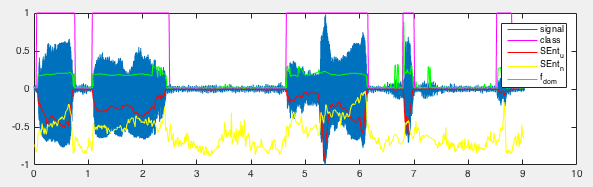
\includegraphics[width=0.6\textwidth]{bilder/VAD_FDsignals.png}
	\caption{Features des Frequenz-Bereiches}
	\label{img:VAD_FDsignals}
\end{figure}

\subsubsection{Cepstrum}

Das \textbf{Cepstrum} wird definiert als die inverse Fourier-Transformation des Logarithmus des Magnituden-Signals nach Formel \ref{eq:cepstrum}.

\begin{equation}
c[n] = F^{-1}\{\log|F\{x[n]\}|\}
\label{eq:cepstrum}
\end{equation}

Die Idee wird anhand von Abbildung \ref{img:cepstrum} verdeutlicht. Zu sehen ist ein typisches absolutes Spektrum eines Signalfensters mit Stimme $|F\{x\}|$. Durch die Logarithmisierung des Spektrums wird die Dynamik der Amplitudenunterschiede eingegrenzt. Das entstandene Signal $\log|F\{x[n]\}|\}$ zeigt klar die Lage der Formanten, dargestellt durch die durchgezogene, schwarze Linie. Die vielen, kleinen Signalspitzen, die sich entlang der Formantenlinie bewegen, sind die harmonsichen Obertöne, die von dem periodischen Signal der Stimmbänder erzeugt wurden. Der Grundgedanke ist, dieses Spektrum wiederum als Signal zu interpretieren. Wäre dieses Signal im Zeitbereich (obwohl es eigentlich den Frequenzbereich darstellt), könnte es durch die Amplituden-Modulation eines Quasi-periodischen Signales entstanden. Das höherfrequente Signal (Spektrum der Stimmbänder) wäre dementsprechend der Träger, und das niederfrequente Signal (Spektrum der Formanten) der Modulator.Um diese beiden Signalanteile voneinander zu trennen, würde man eine weitere Fourier-Transformation implementieren (welche an dieser Stelle mathematisch betrachtet einer inversen Fourier-Transformation gleichkommt, da das Phasensignal entfernt wurde). Man erwartet in dem so entstehenden Spektrum $F^{-1}\{\log|F\{x[n]\}|\}$ eine Spitze im niederfrequenten Bereich, bedingt durch den niederfrequenten Modulator, und eine Spitze im höheren Frequenzbereich, bedingt durch den höherfrequenten Träger. 

Der Bereich dieser \glqq Fouriertransformation der Foueriertransformation\grqq{} wird als \emph{Cepstrum} bezeichnet. Cepstrum ist ein ein Wortspiel, welches durch die Umkehrung der ersten vier Buchstaben des Wortes "Spectrum" ensteht. Die Unabhängige Variable des Cepstrum folgt dem Wortspiel und wird als \emph{Quefrency} bezeichnet. Damit wird verdeutlicht, dass die unabhängige Variable des Cepstrum zwar mathematisch betrachtet die Zeit darstellt, jedoch als Frequenz interpretiert wird.

\begin{figure}[h]
	\centering
	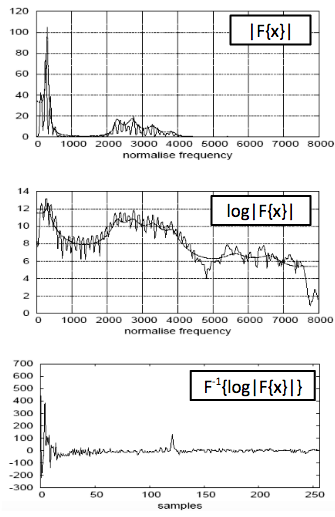
\includegraphics[width=0.6\textwidth]{bilder/Cepstrum02.png}
	\caption{Entstehung des Cepstrums}
	\label{img:cepstrum}
\end{figure}

Insbesondere das Vorhandensein einer Spitze im Quefrency-Bereich ab 3 ms im Cepstrums weist auf das Vorhandensein von harmonischen Obertönen eines periodischen Eingangssignal hin, wie es von Stimmbändern erzeugt wird. Eine Grundfrequenz von $f_0$ dieser periodischen Schwingung entspricht einer Signalspitze bei der Quefrency von $\frac{1}{f_0}$. Abbildung \ref{img:cepstrum2} zeigt das Log-Spektrum und das Cepstrum eines Sprachsignales, welches in Fenster à 50 ms zerlegt wurde. Die Frames 1-7 sind stimmlos, die Frames 8-15 stimmhaft. Die Stimmhaftigkeit spiegelt sich klar im auftauchen einer Signalspitze bei einer Quefrency von 10 ms wieder.\cite{ricardo_ceps}


\begin{figure}[h]
	\centering
	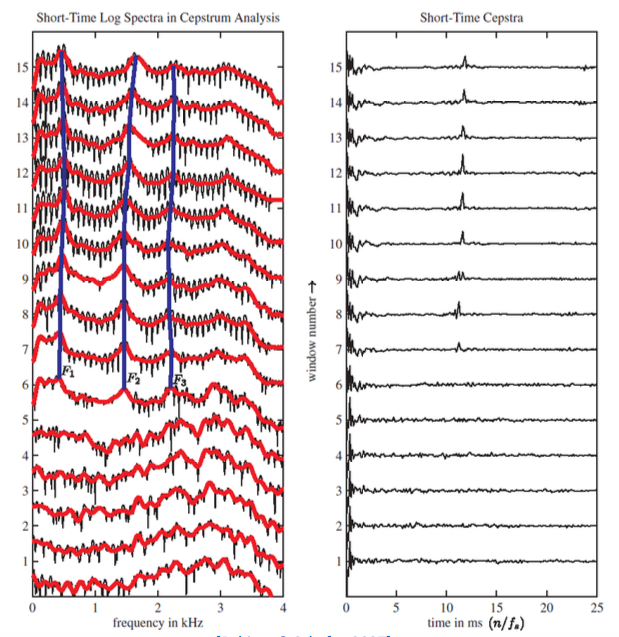
\includegraphics[width=0.6\textwidth]{bilder/Cepstrum03.png}
	\caption{Cepstrum}
	\label{img:cepstrum2}
\end{figure}

Die Informationen des Cepstrum eigenen sich ebenfalls zur Voice-Activity-Detection. Es werden die Features \emph{Upper Cepstrum Peak} $[ Ceps_{mag} ]$ und \emph{Upper Cepstrum Peak Location} $[ Ceps_{loc} ]$ berechnet.

Wie in \cite{vad_ceps} und \cite{vad_Lisboa} beschrieben, wurde die \emph{höchste Magnitude im oberen Quefrency-Bereich} (Upper Cepstrum Peak) nach Formel \ref{eq:ceps_maxpeak} berechnet. Nach \cite{lod} liegt die Grundfrequenz eines Kinderweinens zwischen 250 und \SI{2000}{\hertz}, was einem Quefrency-Bereich von 5 - 40 ms entspricht. Folglich werden bei der Berechnung nach Formel \ref{eq:ceps_maxpeak} nur Quefrency-Werte in diesem Bereich betrachtet werden. Eine hoher $Ceps_{mag}$-Wert weist auf das Vorhandensein von Stimme für das aus dem Fenster $x_i$ Berechneten Cepstrum $x_i$ hin. Als zweites Features des Cepstrums wird die Quefrency der so gefundenen höchsten Magnitude (Upper Cepstrum Peak Location) nach Formel \ref{eq:ceps_loc} berechnet. Bei Signalfenstern mit Stille ist es wahrscheinlicher, dass sich die Spitze am Mindest- oder Maximum-Wert des Cepstrum befindet. 

\begin{equation}
Ceps_{mag}(c_i) = \max_{k}\{\text{mag}(c[k])\}
\label{eq:ceps_maxpeak}
\end{equation}

\begin{equation}
Ceps_{loc}(c_i) = \argmax_{k}\{\text{mag}(c[k])\}
\label{eq:ceps_loc}
\end{equation}

Abbildung \ref{img:VAD_CeDsignals} visualisiert die beiden Features des Cepstrums auf die selbe Art und Weise, wie es bei Abbildung \ref{img:VAD_TDsignals}

\begin{figure}[h]
	\centering
	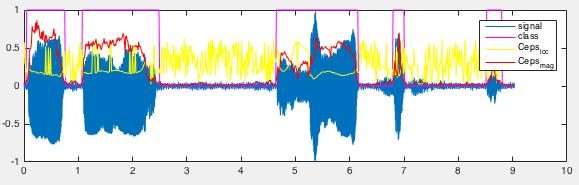
\includegraphics[width=0.6\textwidth]{bilder/VAD_CeDsignals.png}
	\caption{Features des Cepstrums}
	\label{img:VAD_CeDsignals}
\end{figure}

\subsubsection{Autokorrelation}

Die vierte Methode, die zur Voice-Activity-Detection verwendet wird, ist die \textbf{Autokorrelation}. Dabei wird das Signalfenster $x_i$ mit einer verzögerten Variante von sich selber nach Formel \ref{eq:autocorr} korreliert. Der Parameter $k$ wird als Lag bezeichnet und definiert die Verzögerung des Signals, mit dem die Korrelation durchgeführt wird. Ein hoher Autokorrelationswert bei einem bestimmten Lag $k$ weist darauf hin, dass das Signal eine Periodizität bezüglich diesem Verzögerungswert aufweist. Möchte man beispielsweise berechnen, ob ein bei \SI{16000}{\hertz} gesampeltes Signal bezüglich \SI{400}{\hertz} periodisch ist, so wird die Autokorrelation mit einem Lag von $k = \frac{ \text{Sampling-}f_s}{\text{Detect-}f_s}=\frac{\SI{16000}{\hertz}}{\SI{400}{\hertz}} = 40 $ durchgeführt. Formel \ref{eq:normcorr} zeigt die \emph{normalisierte Autokorrelation}, bei der das Autokorrelations-Signal sowohl bezüglich der Signalenergie als auch der Anzahl der Lags normalisiert wird.

\begin{equation}
a_i[k] = \sum_{n=k}^{N}x_i[n] \cdot x_i[n-k]
\label{eq:autocorr}
\end{equation}

\begin{equation}
acorr_i[k] = \frac{\sum_{n=k}^{N}x_i[n] \cdot x_i[n-k]}{\sqrt{(\sum_{n=1}^{N-k}x_i[n]^2)} \cdot\sqrt{(\sum_{n=k}^{N}x_i[n]^2)}}
\label{eq:normcorr}
\end{equation}

Abbildung \ref{img:acorr} zeigt das $acorr_i$-Signal eines Sprachsignals mit den Lags 50 - 320. Die höchste Signalmagnitude bei Lag = 145 ist ein Indikator dafür, dass bei einer Samplingrate von \SI{16000}{\hertz} die Grundfrequenz $\frac{\SI{1600}{\hertz}}{145} = \SI{110,34}{\hertz}$ am dominantesten im Signal enthalten ist, was bei einem Stimmsignal die Grundfrequenz $f_{0}$ ist.

\begin{figure}[h]
	\centering
	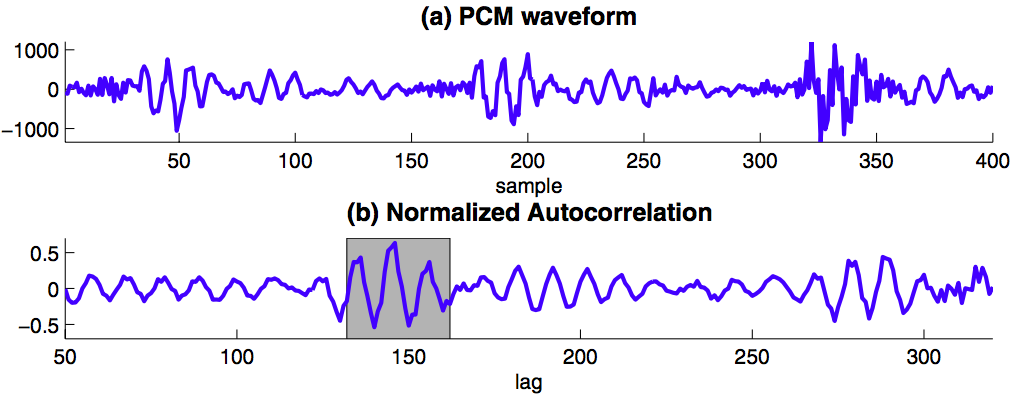
\includegraphics[width=0.6\textwidth]{bilder/acorr.png}
	\caption{Autokorrelation eines Signals}
	\label{img:acorr}
\end{figure}

Da Stimmsignale eine höhere Periodizität aufweisen als das Hintergrundrauschen, eignet sich die Autokorrelation zur Voice-Activity-Detection. Es werden die Features \emph{Maximum Autocorrelation Peak} [\emph{aMax}] und (\emph{Autocorrelation Peak Count}) [\emph{aCount}] berechnet. 

Beide Features werden in \cite{vad_granada} zur VAD verwendet. Die \emph{höchste Magnitude der Autokorrelation }  (\emph{Maximum Autocorrelation Peak}) wird nach der Formel \ref{eq:corrpeak} definiert. Eine höherer \emph{aMax}-Wert weist auf das Vorhandensein von Periodizität im Signal und somit auf Stimme hin. Das zweite Feature ist die \emph{Anzahl an Autokorrelatoins-Spitzen} nach Formel \ref{eq:corrcount}. Da nach \cite{lod} die Grundfrequenz eines Kindergeschreis zwischen 250 und \SI{2000}{\hertz} liegt, wurden auch nur Lags für diesen Bereich verwendet. 

\begin{equation}
\text{aMax}(x_i) = \max_{k}\{\text{mag}(acorr_i[k])\}
\label{eq:corrpeak}
\end{equation}

\begin{equation}
\text{aCount}(x_i) = \counti_{k}\{\text{mag}(acorr_i[k])\}
\label{eq:corrcount}
\end{equation}

Abbildung \ref{img:VAD_CoDsignals} visualisiert die Features der Autokorrelation auf die selbe Art und Weise wie bei Abbildung \ref{img:VAD_TDsignals}.

\begin{figure}[h]
	\centering
	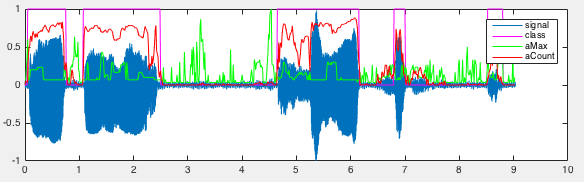
\includegraphics[width=0.6\textwidth]{bilder/VAD_CoDsignals.png}
	\caption{Features der Autokorrelation}
	\label{img:VAD_CoDsignals}
\end{figure}

\subsubsection{Konstruktion des Feature-Vektors}

Für jedes Signalfenster à \SI{25}{\milli\second} werden die 9 vorgestellten Features \emph{RMS, ZCR, SEnt\textsubscript{u}, SEnt\textsubscript{n}, $f_{Dom}$, Ceps\textsubscript{mag}, Ceps\textsubscript{loc}, aMax} und \emph{aCount} berechnet. Wie beschrieben, sollten Signalfenster mit Stimme einen höheren Wert des jeweiligen Features erzeugen als Signalfenster mit Stille (oder, abhängig vom Feature wie der ZCR, einen tieferen). 

Abbildung \ref{img:min-signal} zeigt in (a) die RMS-Werte eines Signals mit einem Signal-Rausch-Abstand (SNR) von \SI{50}{\decibel}. Die Zeiträume mit Stille haben einen weitaus niedrigeren RMS-Wert als die Signalteile mit Stimme. In (b) ist das selbe Signal mit einem Signal-Rausch-Abstand von \SI{3}{\decibel} zu sehen. Nun liegen die RMS-Werte des Rauschens nur noch knapp unter denen des Sprachsignals. Zu sehen ist, dass starkes Hintergrundrauschen ähnlich hohe Feature-Werte erzeugen kann wie die Stimme.

\begin{figure}[h]
	\centering
	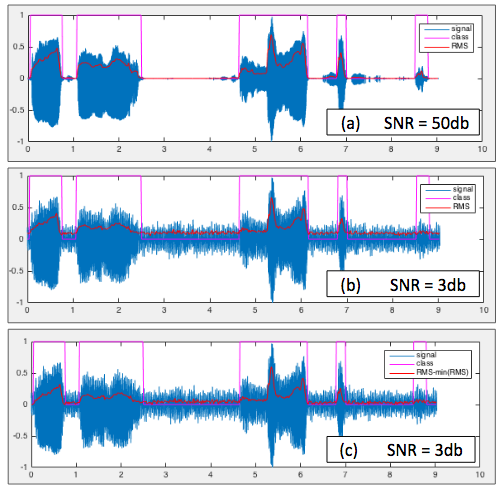
\includegraphics[width=0.6\textwidth]{bilder/min-signal.png}
	\caption{Differenz-Signal des RMS-Wertes}
	\label{img:min-signal}
\end{figure}

In \cite{vad_Easy} und \cite{vad_entropy} wird die Idee präsentiert, den Wert des jeweiligen Features zu messen, der in den stimmlosen Segmenten durch das Hintergrundrauschen erzeugt wird. Jedoch ist für ein Signalfenster $x_i$ zum Zeitpunkt der Berechnung des Features noch nicht bekannt, ob es sich um ein Zeitfenster mit Stille oder Stimme handelt. Genau diese Entscheidung wird später auf Basis der Features getroffen. Man kann jedoch davon ausgehen, dass kein Baby-Schrei länger eine bestimmte Zeitraum $t_{max}$ dauert, bevor das Babie Luft holen muss und somit ein Zeitfenster mit Stille entsteht. Der Mindestwert eines Features in einem Zeitraum  $t_{max}$ ist somit der Wert des Features, der mindestens durch das Hintergrundrauschen erzeugt wird. Er wird nach Formel \label{ref:minFeat} berechnet, wobei $t_{xi}$ die Länge eines Signalfensters $x_i$ ist (in diesem Fall \SI{25}{\milli\second}). Das \emph{Differenzfeature} wird definiert nach Formel \ref{eq:difFeature} als die Differenz des für das aktuelle Signalfenster berechneten Features und dem Mindestwert dieses Feature der letzten $t_{max}$ Sekunden.

\begin{equation}
\text{MinF}(Feat(x_i)) = \min_{k=i-z...i}( \text{Feat}(x_k)), z = \frac{2 t_{max}}{t_{xi}}
\label{eq:minFeat}
\end{equation}

\begin{equation}
\text{DiffF}(Feat(x_i)) = Feat(x_i) - MinF(Feat(x_i))
\label{eq:difFeature}
\end{equation}

Der Featurevektor, der schlussendlich für jedes Signalfesnter $x_i[]$ berechnet wurde, besteht neben den 9 vorgestellten Features, zusätzlich aus den Differenzfeatures für einen Zeitraum von $t_{max} = 4$ Sekunden. Features, deren Wert bei Stimmhaften Signalfenstern geringer ist als bei stimmlosen, werden an der x-Achse gespiegelt, um Formel \ref{eq:minFeat} anwenden zu können (das Betrifft die Features ZCR, SEnt\textsubscript{u} und aCount). Das einzige Feature, welches nicht als Differenzfeature dem Feautrevektor beigefügt wurde, ist der \emph{Upper Cepstral Peak Location}-Feature [$Ceps_{loc}$], da es bei Stille sowohl einen höheren als auch einen niedrigeren Wert annehmen kann. Der Feature-Vektor $V$ des Signalfensters $x_i$ wird nach Formel \ref{eq:featureVektor} berechnet umfasst 17 Features, wobei 9 absolute Features und 8 Differenzfeatures verwendet werden.

\begin{equation}
\begin{split}
V(x_i) = \Big( \text{RMS}(x_i), ...,\text{ aCount}(x_i)\\
\text{DiffF}(\text{RMS}(x_i)) .... \text{DiffF}(-\text{ aCount}(x_i))\Big)
\end{split}
\label{eq:featureVektor}
\end{equation}

\subsection{Thresholding}

\subsubsection{Finden der Grenzwerte}

Für jedes Signalfenster $x_1...x_n$ liegt nun ein Featurevektor $v_1...v_n$ vor. Das Ziel ist nun, Grenzwerte für die Features zu finden, bei deren Überschreitung das Signalfenster als \emph{Stimmhaft} kategorisiert wird. Abbildung \ref{img:thresholded} verdeutlicht das Prinzip für das Feature \emph{Ceps\textsubscript{mag}}. Eine binäre Kategorisierung nach dem Muster $C(x_i) = \{ 1, \text{wenn} \text{ Ceps}_{mag}(x_i) \geq 0.2 , 0 \text{ sonst}\}$ würde auf den ersten Blick eine weitgehend richtige Kategorisierung vornehmen.

\begin{figure}[h]
	\centering
	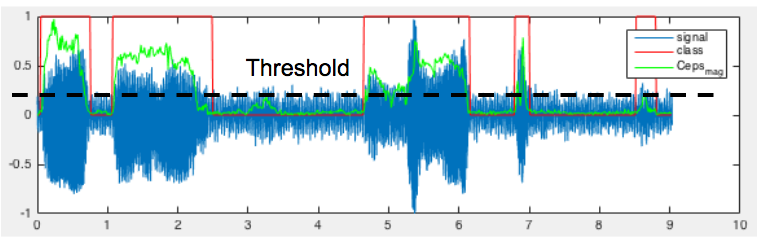
\includegraphics[width=0.6\textwidth]{bilder/thresholded.png}
	\caption{Thresholding eines Feature-Signales}
	\label{img:thresholded}
\end{figure}

Es sind  Kombinationen von Grenzwerten in Form von Entscheidungsbäumen denkbar, wenn mehrere Features in die Kategorisierung einfließen. Ein Beispiel wird in Listing \ref{lst:tree01} dargestellt, bei dem die Kategorsierung hierarchisch zuerst nach einem Grenzwert für Ceps$_{mag}$ und danach für den RMS-Wert entschieden wird.


\begin{lstlisting}[frame=single,mathescape=true,basicstyle=\footnotesize,language=Java,label=lst:tree01,caption=Beispiel eines CART-Entscheidungsbaums,linewidth=1\textwidth]
if Ceps$_{mag}$($x_i$) > 0.2
|   if RMS($x_i$) < 0.13
|   |   C($x_i$) = 0
|   |else
|   |   C($x_i$) = 1
|else
|    C($x_i$) = 1
\end{lstlisting}


Zur Festlegung der Grenzwerte wird ein \emph{Classification And Regression Tree} (CART)-Algorithmus verwendet. CART-Algorithmen sind Klassifizierungsalgorithmen, bei denen Entscheidungsbäume wie in Listing \ref{lst:tree01} konstruiert werden. Sie haben den Vorteil, dass die Klassifizierung in Form von Regeln mit Grenzwerten dargestellt werden können, die für den Menschen nachvollziehbar sind (im Gegensatz zu z.B. Neuronalen Netzen). Der durch den CART-Algorithmus konstruierte Entscheidungsbaum wird auch als \emph{Klassifizierungs-Modell} bezeichnet.\cite{id3}

Einer der bekanntesten CART-Algorithmen ist der ID3-Algorithmus, entwickelt von J. Ross Quinlan an der University of Sidney. Als Trainingsdatensatz $S$ wird eine Menge an Instanzen verwendet, deren Klassenzugehörigkeit bereits bekannt ist. Der ID-3 Algorithmus funktioniert nur für diskrete Features und Klassen. Ein Beispiel für ein diskretes Feauture ist [\emph{Lautstärke = \{laut, leise\}}]. Ein Beispiel für ein numerisches Feature, welches vom ID-3 Algorithmus nicht akzeptiert wird, ist [\emph{Lautstärke =} $\mathbb{N}$]. Der Algorithmus funktioniert folgendermaßen:
\begin{enumerate}
	\item Gehören alle Instanzen des Datensatzes $S$ nur einer Klasse an?
	\begin{enumerate}
		\item Ja: Markiere diesen Knoten als Blatt und STOP. 
		\item Nein: Erzeuge einen neuen Knoten. Wähle das Feature $F$, welches den höchsten \emph{Informationsgewinn} bringt. Das heisst, dass dieses Feature die stärkste Unterscheidung zwischen den einzelnen Klassen ermöglicht. Der Informationsgewinn $H(S)$ eines Features $F$ mit den Untermengen $X$, welche aus den Instanzen der selben Klasse bestehen, wird mit Hilfe der Entropie nach Formel \ref{eq:entropie} berechnet.
	\end{enumerate}
	
	\begin{equation}
	H(S) = -\sum_{x \in X} F(x) \log_2 F(x)
	\label{eq:entropie}
	\end{equation}
	
	\item Unterteilung den Trainingsdatensatz $S$ in die Untermengen $S_1 ... S_n$, wobei eine Untermenge für jeden möglichen Attributbwert des ausgewählten Features gebildet wird. 
	
	\item Wiederhole die Schritte 1. und 2. für alle Untermengen $S_1...S_n$ \cite{id3}
	
\end{enumerate}

Der C.45-Algorithmus ist eine Erweiterung des ID-3 Algorithmus, der neben anderen Erweiterungen ebenfalls mit numerischen Attributwerten umgehen kann. Dafür werden für ein Feature alle Instanzen des Datensatzes $S$ nach den Werten dieses Features geordnet und derjenige Grenzwert gesucht, der den höchsten Informationsgewinn bringt. Der Datensatz wird daraufhin an den Knoten in genau 2 Untermengen  aufgespalten.\cite{c45} 

Zum Finden der Grenzwerte der in Kapitel \ref{sec:featExtraction} beschriebenen Features wurde die Implementierung des C.45-Algorithmus \emph{REPTree}\footnote{Dokumentation von REPTree: \url{http://weka.sourceforge.net/doc.dev/weka/classifiers/trees/REPTree.html}} der Open Source Data-Mining-Bibliothek \emph{Weka}\footnote{Download von WEKA: \url{http://www.cs.waikato.ac.nz/ml/weka/}} verwendet. Diese hat den Vorteil, dass die Tiefe des Entscheidungsbaumes festlegbar ist und somit die Komplexität des Baumes begrenzt werden kann. Ein Nebeneffekt ist, dass so Overfitting, also die Überanpassung des Entscheidungsbaumes auf den Trainingsdatensatz, vermieden wird.

\subsubsection{Trainings- und Testdatensätze}
\label{sec:databases}

Zum Training des REPTree-Algorithmus musste in Trainingsdatensatz $S$ erstellt werden. Dazu wird zunächst eine Menge an Audiosignalen benötigt. Es wurden 6 Audiosignale mit Weinen von Babies von der freien Online-Sound-Bibliothek \url{https://www.freesound.org/} heruntergeladen und zu Segmenten à 10 Sekunden beschnitten. Diese Audiosignale sind weitestgehend Rausch-frei. Die Segmente der Audiosignale wurden händisch Kategorisiert in die Klassen \{1 = Stimme, 0 =  Still\}. Weiterhin wurden 3 verschiedene Rauschsignale heruntergeladen. Es handelt sich um "realistische" Rauschsignale mit Krankenhausatmosphären. Jedes dieser 3 Rauschsignale wurde mit den 6 Weinsignalen überlagert, einmal mit einem Signal-Rausch-Abstand von \SI{50}{\decibel} (fast unhörbares Rauschen), und einmal mit einem Signal-Rausch-Abstand von \SI{3}{\decibel} (sehr starkes Rauschen). Außerdem wurde ein Testsignal erzeugt, welches eine siebte Tonaufnahme eines Kinderweinens enthält, dass mit einem vierten Rauschsignal mit einem SNR von \SI{7}{\decibel} überlagert wurde. Dieses Signal spielt eine Sonderrolle, da es nur zur Verifikation verwendet wird und enthält daher nur ein Audiosignal (Siehe Kapitel \ref{sec:results}) So wurden vier Mengen an Audiosignalen erzeugt:

\begin{description}
	\item[A\textsubscript{\SI{50}{\decibel}}] enthält $3 \cdot 6=18$ Audiosignale, bei dem alle 6 Wein-Signale mit den 3 Rauschsignalen bei einem Signal-Rausch-Abstand von \textbf{\SI{50}{\decibel}} überlagert wurden
	
	\item[A\textsubscript{\SI{3}{\decibel}}] enthält $3 \cdot 6=18$ Audiosignale, bei dem alle 6 Wein-Signale mit den 3 Rauschsignalen bei einem Signal-Rausch-Abstand von \textbf{\SI{3}{\decibel}} überlagert wurden
	
	\item[A\textsubscript{50+\SI{3}{\decibel}}] $ = \{ A_{\SI{50}{\decibel}} \cup  A_{\SI{3}{\decibel}}\} = 32$ Audiosignale
	
	\item[A\textsubscript{\SI{7}{\decibel}*}] enthält $1$ Audiosignal, bei dem ein siebstes Wein-Signale mit einem vierten Rauschsignal bei einem Signal-Rausch-Abstand von \textbf{\SI{7}{\decibel}} überlagert wurde.
	
\end{description}

Im nächsten Schritt werden die eigentlichen Trainingsdatensätze $S_{SNR,Feat}$ gebildet, in dem Audiosignale dieser Signalmengen (1) wie in Kapitel \ref{sec:preprocessing} vorverarbeitet werden, (2) wie in Kapitel \ref{sec:windowing} in die Signalfenster à \SI{25}{\milli\second} zerlegt werden und (3) für jedes Audiosignal die durch Gleichung \ref{eq:featureVektor} definierte Featurevektoren berechnet werden. Außerdem wird jedem Featurevektor die Klasseninformation \emph{Stimme/Stille} zum Training des REPTree-Algorithmus mitgegeben. 

Es ist rechnerisch zu Aufwendig, alle genannten Features in einem kontinuierlichen System zur Voice Activity Detection zu berechnen. Daher werden Untermengen der Features in den Datensätzen gebildet. Das Ziel ist es, diejenige Untermenge an Features zu finden, die sich am besten für die Voice-Activity-Detection sowohl bei niedrigem als auch bei starkem Hintergrundrauschen eignet. Die Untermengen werden in Bezug auf die Methode gebildet, durch die die Features berechnet werden. Das heißt, dass beispielsweise die Untermenge \emph{Zeit} die in Kapitel \ref{sec:timeFeats} beschriebenen Features \emph{RMS} und \emph{ZCR} sowie die dazugehören Differenzfeatures \emph{FDiff(RMS)} und \emph{FDiff(ZCR)} beinhaltet. 

Die 9 Untermengen sind: \{ Zeitbereich, Frequenzbereich, Cepstrum, Autokorrelation, Zeit + Frequenzbereich, Zeit + Cepstrum, Zeit + Autokorrelation, Frequenz + Cepstrum, Frequenz + Autokorrelation \}. 

So enthält beispielsweise der Datensatz $S_{\SI{3}{\decibel},Zeit}$
die Featurevektoren des Zeitbereiches für die Audiosignale mit einem Signal-Rausch-Abstand von 3\SI{25}{\decibel}. Die Audiosignal-Mengen [A\textsubscript{\SI{50}{\decibel}}], [A\textsubscript{\SI{3}{\decibel}}] [A\textsubscript{50+\SI{3}{\decibel}}] und [A\textsubscript{\SI{7}{\decibel}* }] wurden in Datensätze umgewandelt. Es werden schlussendlich $4 \cdot 9 = 36$ Datensätze gebildet.

\subsubsection{Training und Ergebnis} 
\label{sec:results}

Der REPTree-Algorithmus entwirft einen Entscheidungsbaum, der für den angegebenen Trainingsdatensatz eine möglichst hohe Accuracy gewährleistet (unter den gegebenen Einschränkungen eines CART-Algoirthmus). Wird dem REPTree-Algorithmus beispielsweise der Datensatz $S_{\SI{3}{\decibel},Zeit}$ (also der Datensatz mit einem SNR von \SI{3}{\decibel} unter Verwendung der Zeit-Features, siehe Kapitel \ref{sec:databases}) als Input gegeben, entwirft der Algorithmus einen Entscheidungsbaum auf Basis dieses Datensatzes. Wird das gebildete Modell daraufhin für die Klassifikation der A\textsubscript{\SI{3}{\decibel}}-Signalmenge verwendet, kann man aus dem Klassifikationsergebnis die Accuracy des Modells für diesen Signal-Rausch-Abstand berechnen. 

Der Datensatz $S_{SNR,Feat}$, der als Input für den REPTree-Algorithmus und somit zur Bildung des Entscheidungsbaums verwendet wird, wird als \emph{Trainings-Datensatz} bezeichnet. Die Signalmenge $A_{SNR}$, auf den das Modell angewandt wird und für den die Accuracy berechnet wird, wird als \emph{Test-Datensatz} bezeichnet. Wird also beispielsweise der Trainings-Datensatz $S_{\SI{50}{\decibel},Zeit}$ und als Test-Signalmenge $A_{\SI{3}{\decibel}}$ verwendet, so kann man berechnen, wie gut sich ein Modell unter Verwendung der Zeit-Features zur Klassifizierung niedriger SNRs eignet, obwohl es für hohe SNRs entworfen wurde.

Das Ziel ist, den Entscheidungsbaum für eine Feature-Untermenge zu finden, die eine möglichst hohe Klassifikations-Accuracy für sowohl hohe als auch niedrige SNR gewährleistet. Die Frage ist, ob ein Entschiedungsbaum, der für einen niedrigen SNR gebildet wird, auch für hohe SNR gut funktioniert, oder ob das Gegenteil zutreffend ist. Daher werden die Entscheidungsbäume sowohl auf Basis verschiedener SNRs als auch verschiedener Feature-Untermengen gebildet. Die Modelle werden daraufhin gegen die Signale mit den hohen und niedrigen SNRs getestet.

Es wurden, wie in Kapitel \ref{sec:databases} beschrieben, $3 \cdot 9 = 27$ Trainings-Datensätze erzeugt ( [3 SNR-Werten: \SI{3}{\decibel}, \SI{50}{\decibel} und 50+\SI{3}{\decibel} ] $\times$ [9 Feature-Untermengen]. Der Datensatz mit einem SNR von \SI{7}{\decibel} wird \emph{nicht} zum Training verwendet). Mit diesen 27 Trainingsdatensätze werden mit Hilfe des REPTree-Algorithmus 27 Klassifikationsbäume erzeugt. Jeder Klassifikationsbaum wurde gegen die 3 Testdatensätze A\textsubscript{\SI{3}{\decibel}}, A\textsubscript{\SI{50}{\decibel}} und A\textsubscript{\SI{7}{\decibel}*} getestet und die Accuracy berechnet. Das Signal A\textsubscript{\SI{7}{\decibel}*} erfüllt dabei eine Sonderrolle, da weder das Signal des Weinens noch das Rausch-Signal in den Trainingsdatensätzen enthalten sind und somit verifiziert wird, ob der Datensatz nur \glqq auswendig gelernt\grqq{} wird oder das Modell auf neue Anwedungsfälle übertragen werden kann. Um Overfitting des Modells zu vermeiden und die Komplexität des Entscheidungsbaumes zu verringern, wurde die maximale Tiefe des REPTree auf 2 gesetzt. Die Ergebnisse sind in Tabelle \ref{tab:reptree_results} zu sehen.

Die Features, welche zu den höchsten Accuracy-Werten führten, sind die des \emph{Cepstrum}-Bereiches, genauer gesagt das DiffF(Ceps\textsubscript{mag})-Feature, da es vom REPTree-Algorithmus als einziges Feature dieses Bereiches für die Entscheidungsbäumen ausgewählt wurde. Die Entscheidungsbäume, die mit dem DiffF(Ceps\textsubscript{mag})-Feature entworfen wurden, erreichten eine durchschnittliche Accuracy (das heißt, gemittelt über die Testsignale A\textsubscript{\SI{3}{\decibel}}, A\textsubscript{\SI{50}{\decibel}} und A\textsubscript{\SI{7}{\decibel}*}) von mindestens 91,45\%. Der nächstbeste Entscheidungsbaum mit einer Accuracy von 86,96\% wurde unter Verwendung der Features des Zeitbereiches und der rechnerisch aufwendigeren Autokorrelation auf dem Datensatz S\textsubscript{50+\SI{3}{\decibel},Zeit+Correlation} entworfen. Sobald der Cepstrum-Bereich in Verbindung mit den Features der Bereiche \emph{Zeit} und \emph{Frequenz} verwendet wurde, wurde das DiffF(Ceps\textsubscript{mag})-Feature vom REPTree-Algorithmus bevorzugt, so dass die Features der anderen beiden Bereiche keine Anwendung mehr in den entsprechenden Bäumen fanden.

Auf Basis der Datensätze S\textsubscript{\SI{3}{\decibel},Ceps}, S\textsubscript{\SI{3}{\decibel},Zeit+Ceps}, S\textsubscript{\SI{3}{\decibel},Freq+Ceps}, S\textsubscript{50+\SI{3}{\decibel},Ceps}, S\textsubscript{50+\SI{3}{\decibel},Zeit+Ceps} sowie \linebreak S\textsubscript{50+\SI{3}{\decibel},Freq+Ceps} wurde der selbe Entscheidungsbaum erzeugt, der in Listing \ref{lst:cepsTree01} zu sehen ist. Auf Basis der Datensätze S\textsubscript{\SI{50}{\decibel},Ceps} und S\textsubscript{\SI{50}{\decibel},Zeit+Ceps} wurde der Entscheidungsbaum in Listing \ref{lst:cepsTree02} erzeugt. Es ist zu sehen, dass (a) beide Entscheidungsbaum einen einfachen Grenzwert für das DiffF(Ceps\textsubscript{mag})-Feature setzen, und zweitens (b) sich die beiden Modelle nur im konkreten Wert des Grenzwertes unterscheiden. 

Da das Modell aus Listing \ref{lst:cepsTree01} eine durchschnittliche Accuracy von 92,22\% und das Modell aus Listing \ref{lst:cepsTree02} eine unwesentlich geringere Accuracy von 91,45\% erreicht, wurden für beide Modelle die Specificity und Sensitivity berechnet, um eine Entscheidung für eines der beiden Modelle fällen zu können. Dazu wurden die Signalmengen A\textsubscript{\SI{3}{\decibel}}, A\textsubscript{\SI{50}{\decibel}} und A\textsubscript{\SI{7}{\decibel}*} in Frames à 100 Windows zerlegt und für jedes Zeitfenster die Senstivity, Specificity und Accuracy bezüglich der beiden Modelle berechnet. Die Ergebnisse werden als Boxplots in Abbildung \ref{img:boxplots} dargestellt. Der Unterschied zwischen den Modellen ist am Stärksten beim Testing gegen die Signale mit einem SNR von \SI{3}{\decibel} und \SI{7}{\decibel}  zu sehen. Das Modell mit dem Grenzwert von 0.03 erzielt in beiden Fällen eine höhere Specificity, aber geringere Senstivitiy als das Modell mit dem Grenzwert bei 0.02. Es wurde sich für das Modell für mit einem Grenzwert von 0.02 entschieden, da durch die höhere Senstivity mehr Wein-Signale erkannt werden, die in späteren Verarbeitungsschritten immernoch als False-Positives erkannt und verworfen werden können. Einmal im Prozess der VAD als Stimmlos markierte Fenster werden jedoch nicht weiter verarbeitet und gehen somit \glqq verloren\grqq. 

\begin{minipage}{\linewidth}
	\begin{lstlisting}[frame=single,mathescape=true,basicstyle=\footnotesize,language=Java,label=lst:cepsTree01,caption=Entscheidungsbaum für die VAD mit einem Cepstrum-Grenzwert von 0.02,linewidth=1\textwidth]
	if FDiff(Ceps$_{mag}$($x_i$)) < 0.02
	|   C($x_i$) = 0
	|else
	|   C($x_i$) = 1
	\end{lstlisting}
\end{minipage}

\begin{minipage}{\linewidth}
	\begin{lstlisting}[frame=single,mathescape=true,basicstyle=\footnotesize,language=Java,label=lst:cepsTree02,caption=Entscheidungsbaum für die VAD mit einem Cepstrum-Grenzwert von 0.03,linewidth=1\textwidth]
	if FDiff(Ceps$_{mag}$($x_i$)) < 0.03
	|   C($x_i$) = 0
	|else
	|   C($x_i$) = 1
	\end{lstlisting}
\end{minipage}

Der Finale Funktion zur Klassifikation eines Signalfensters C$(x)$ in $0 = Stille$ oder $1=Stimme$ ist somit durch Gleichung  \ref{eq:vad-final} gegeben.

\begin{equation}
C(x)=
\begin{cases}
1, & \text{if}\ \text{Ceps}_{mag}(x) >= 0.02 \\
0, & \text{otherwise}
\end{cases}
\label{eq:vad-final}
\end{equation}

\subsection{Markierung der Cry-Units}
\label{sec:CryUnit}

Das Ergebnis der Voice-Activity-Detection ist eine Zurdnung aller Signalfenster $x_1 ... x_n$ zu den Klassen $C(x_i) = 0$ \emph{Stille} oder  $C(x_i) = 1$ \emph{Stimme}. In \cite{vad_entropy} wird die Idee vorgestellt, zusammenhängende und ununterbrochene Ketten als \emph{stimmhaft} klassifizierter Signalfesnter zu \emph{Stimm-Segmenten} zusammenzufassen, welche in diesem Zusammenhang eine \emph{Cry-Units} entsprechen. Abbildung \ref{img:cryUnit} veranschaulicht diese Gruppierung. Formel \ref{eq:cry-Unit} gibt die Definition des Datentypes \emph{Cry-Unit} $[CU]$. Eine Cry-Unit definiert sich durch einen Anfangszeitpunkt $start$, einen Endzeitpunkt $end$ und der Liste seiner Signalfenster $windows = [x_1 ... x_n]$.

\begin{figure}[h]
	\centering
	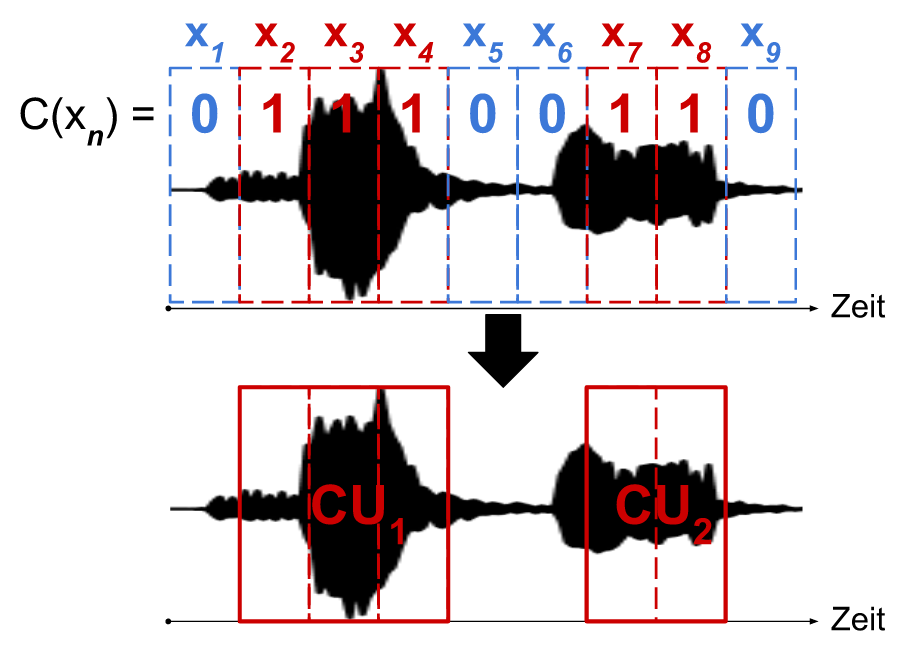
\includegraphics[width=0.6\textwidth]{bilder/cry-Unit01.png}
	\caption{Zusammenfassung klassifizierter Signalfenster zu Cry-Units}
	\label{img:cryUnit}
\end{figure}

Algorithmus \ref{alg:cryUnit} zeigt in Pseudo-Code, wie in der Liste aller Signalfenster $X_{windows} = [x_1 ... x_n]$ eine Liste von Cry-Units $CU_{all} = [cu_1 ... cu_m]$ markiert wird. Die Funktion C$(x)$ ist die Klassifikations-Funktion der Signalfenster in Stille/Stimme nach Gleichung \ref{eq:vad-final}. Die Funktion getTimeOf$(x)$ liefert die Anfangszeitpunkt des Signalfensters $x$.

\begin{equation}
CU = (windows = [x_1 ... x_n ], start \in Zeit, end \in Zeit)
\label{eq:cry-Unit}
\end{equation}

\begin{equation}
\lambda (CU) = CU.end - CU.start
\label{eq:cry-Lambda}
\end{equation}

\begin{equation}
\text{d}(CU_i, CU_j) = CU_j.start - CU_i.end
\label{eq:cry-distance}
\end{equation}

Die Dauer eine Cry-Unit $\lambda(CU)$ wird nach Formel \ref{eq:cry-Lambda} berechnet. Der (Stille)-Zeitraum zwischen zwei Cry-Units d($CU_i, CU_j$), wird nach Formel \ref{eq:cry-distance} berechnet. Diese Zusammenhänge werden in Abbildung \ref{img:cryUnit-details} visualisiert.\cite{vad_entropy}

\begin{figure}[h]
	\centering
	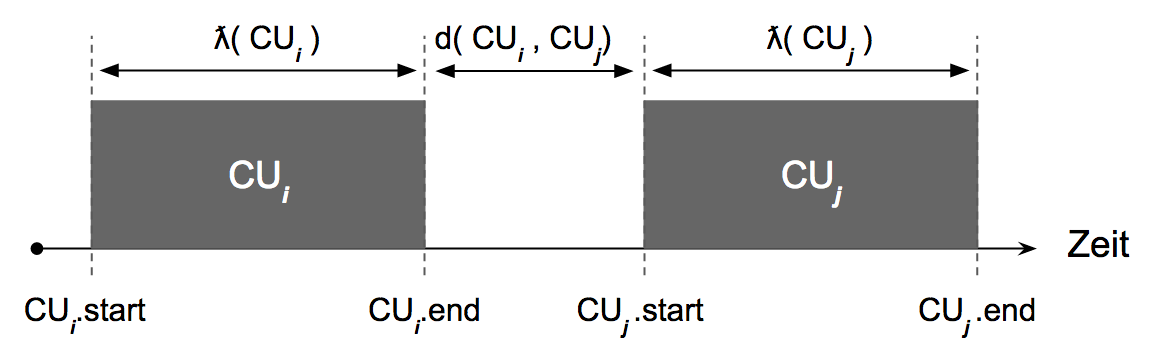
\includegraphics[width=0.6\textwidth]{bilder/newSmoothing03.png}
	\caption{Beziehung zwischen agrenzenden Segmenten}
	\label{img:cryUnit-details}
\end{figure}

\begin{algorithm}[H]
	\caption{Gruppierung von x-Windows zu Cry-Units}
	\label{alg:cryUnit}
	\begin{algorithmic}[1]
		\Function{turnWindowsIntoCryUnits}{$X_{windows}$}
		\State $ CU_{all} \gets []$
		\State $ cu_i \gets ([],0,0)$
		\For{ $i = 1...length(X_{windows})$}
		\State $ c_i \gets C(x_i)$
		\State \Comment Start of Cry-Unit
		\If {$c_i == 1 \wedge \text{isEmpty}(cu_i.windows)$}
		\State $cu_i.start \gets \text{getTimeOf}(x_i)$
		\State $cu_i.windows \gets [cu_i.windows, x_i]$
		\EndIf
		\State \Comment Inside Cry-Unit
		\If {$c_i == 1 \wedge \text{ ! isEmpty}(cu_i.windows)$}
		\State $cu_i.windows \gets [cu_i.windows, x_i]$
		\EndIf
		\State \Comment End of Cry-Unit
		\If {$c_i == 0 \wedge \text{ ! isEmpty}(cu_i.windows)$}
		\State $cu_i.end \gets  getTimeOf(x_i)$
		\State $CU \gets [CU, cu_i]$
		\State $cu_i.windows \gets []$
		\EndIf
		\EndFor
		
		\State \Comment End last Cry-Unit by force if still open.
		\If {$\text{ ! isEmpty}(cu_i.windows) == 0$}
		\State $cu_i.end \gets  getTimeOf(X_{windows}[end])$
		\State $CU_{all} \gets [CU_{all}, cu_i]$
		\EndIf
		
		\Return $CU_{all}$
		
		\EndFunction
		
	\end{algorithmic}
\end{algorithm}

\subsection{Decision Smoothing}

Abbildung \ref{img:beforeSmoothing} zeigt ein Audiosignal mit einem Signal-Rausch-Abstand von \SI{3}{\decibel}, bei dem die Klassifizierung nach dem Entscheidungsbaum aus Listing \ref{lst:cepsTree01} durchgeführt wurde. Die rote Linie zeigt die tatsächliche Klassifizierung, und die grüne Linie die gefundene Klassifizierung nach dem vorgestellten Algorithmus. Die tatsächlichen/gefunden Cry-Units sind klar zu erkennen als die Bereiche, die von der roten/grünen Linie überspannt werden. Es ist zu sehen, dass False-Negatives und False-Positives in der Klassifizierung enthalten sind. Im folgenden werden drei charakteristische Arten falscher Klassifizierungen näher erläutert:
\begin{description}
	\item [False Negatives nach (a) :] Eine korrekt erkannte, längere Cry-Unit wird zu früh beendet. Oft werden kurz nach dem Ende sehr kurze Cry-Units erkannt, die eigentlich noch zu der längeren, vorhergehenden Cry-Unit gehören.
	\item [False Positives nach (b): ] Kurze Cry-Units werden in eigentlichen Stille-Bereichen erkannt.
	\item [False Negatives nach (c): ] Eine Cry-Unit zerfällt in zwei kürzere Cry-Units, da einige Signalfenster in der Mitte als Stille erkannt wurden.
\end{description}

\begin{figure}[h]
	\centering
	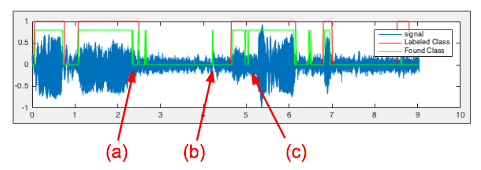
\includegraphics[width=0.6\textwidth]{bilder/smoothing02.png}
	\caption{Klassifizierung vor dem Decision Smoothing}
	\label{img:beforeSmoothing}
\end{figure}

Im Process des \textbf{Decision Smoothing} werden kontextuelle Informationen genutzt, um nachträglich False-Positives und False-Negatives zu entfernen. Es werden dazu die in \cite{vad_entropy} präsentierten Ideen verwendet. Es werden zwei Parameter eingeführt: $\lambda_{min}$, die Mindestlänge einer akzeptierten Cry-Unit, und d$_{min}$, die Mindestlänge eines akzeptierten Stille-Segmentes. Das Decision Smoothing wird nach den folgenden Entscheidungsregeln durchgeführt:

\noindent\rule{\linewidth}{0.3pt}
\begin{itemize}
	\item ist $\lambda (CU_{i}) \leq \lambda_{min}$ ?
	\begin{itemize}
		\item wenn $\lambda (CU_{i-1}) > \lambda_{min}$ und $d (CU_{i-1}, CU_{i}) \leq d_{min}$, dann vereinige $CU_{i}$ mit $CU_{i-1}$ . $\Rightarrow$ behebt False-Negatives des Types (a)
		\item ansonsten entferne $CU_i \Rightarrow$ behebt False-Negatives des Types (b)
	\end{itemize}
	\item wenn $\lambda (CU_{i} > \lambda_{min}$ und $d (CU_{i-1}, CU_{i}) \leq d_{min}$, dann vereinige $CU_{i}$ mit $CU_{i-1}$ . $\Rightarrow$ behebt False-Negatives des Types (c)
\end{itemize}
\noindent\rule{\linewidth}{0.3pt}

Die Entscheidungsregeln greifen Algorithmus greifen nur auf die aktuellen und die letzten bekannte Cry-Unit um, um eine kontinuierliche Analyse zu gewährleisten, weshalb die Entscheidungsregeln jedoch auch komplex sind. Bei einer offline-Analyse können die Entscheidungsregeln vereinfacht werden, da False-Negative Type (a) und (c) mit der selben Regeln abgefragt werden können. Algorithmus \ref{alg:decisionSmoothing} zeigt in Pseudo-Code, wie das Decision-Smoothing durchgeführt wird. Input der Funktion ist die Liste aller Cry-Units $CU_{all}$, die durch Algorithmus \ref{alg:cryUnit} entstanden ist, sowie die Grenzwerte $\lambda_{min}, d_{min}$. Ausgang der Funktion ist die Liste aller Cry-Units nach dem Decision-Smoothing $CU_{smoothed}$.

\begin{algorithm}[H]
	\caption{Decision-Smoothing of VAD}
	\label{alg:decisionSmoothing}
	\begin{algorithmic}[1]
		\Function{decisionSmoothing}{$CU_{all}, \lambda_{min}, d_{min}$}
		\State $CU_{smoothed} \gets[CU_{all}[1]] $
		\For{ $i = 2...length(CU_{all})$}
		\State $cu_i \gets CU_{all}[i]$
		\State $cu_{i-1} \gets CU_{smoothed}[end]$
		\If{$\lambda(cu_i) > \lambda_{min}$}
		\If{d$(cu_{i-1},cu_{i}) > d_{min}$}
		\State $CU_{smoothed} \gets [CU_{smoothed}, cu_i] $
		\Else
		\State \Comment Erase False-Negative Type (c)
		\State $cu_i \gets \text{vereinige}(cu_i, cu_{i-1})$
		\State $CU_{smoothed} \gets [CU_{smoothed}[1:end-1], cu_i] $
		\EndIf
		\Else
		\State \Comment Erase False-Negative Type (a)
		\If{$\lambda(cu_i) > \lambda_{min} \wedge  d(cu_{i-1},cu_{i}) \leq d_{min}$ }
		\State $cu_i \gets \text{vereinige}(cu_i, cu_{i-1})$
		\State $CU_{smoothed} \gets [CU_{smoothed}[1:end-1], cu_i] $
		\Else
		\State \Comment Don't accept $cu_i$. Erases False-Positives (b)
		\EndIf
		\EndIf
		\EndFor
		
		\Return $CU_{smoothed}$
		\EndFunction
		
	\end{algorithmic}
\end{algorithm}

Abbildung \ref{img:after-smoothing} zeigt das Signal vor und nach dem Decision-Smoothing. Die Parameter wurden experimentell mit $\lambda_{min} = 50 ms$ und $d_{min} = 50 ms$ bestimmt.

\begin{figure}[h]
	\centering
	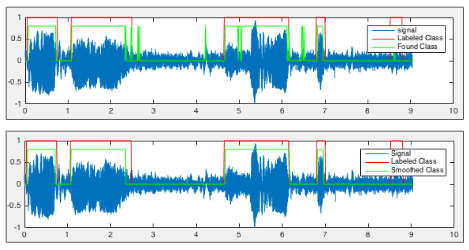
\includegraphics[width=0.6\textwidth]{bilder/smoothing04.png}
	\caption{Klassifizierung vor und nach dem Decision Smoothing}
	\label{img:after-smoothing}
\end{figure}

\section{Segmentierung}

Das Ergebnis der Voice-Activiy-Detection ist eine Liste an Cry-Units  $CU_1 ... CU_n$. Das Ziel ist nun, diese Cry-Units zu Cry-Segmenten zu gruppieren. Ein Cry-Segment definiert sich nach Golub et al \cite{cryModel} als \glqq die komplette klangliche Antwort auf einen spezifischen Stimulus. Sie kann mehrere Cry-Units entahlten \grqq . Die Defintion lässt folgende Fragen offen:

\begin{itemize}[leftmargin=*]
	\item Beginnt das Segment bereits bei Zuführung des Stimulus, oder erst ab der ersten Cry-Unit? 
	\item Wodurch definiert sich der Beginn, wenn ohne Zuführung eines Stimulus das Baby beginnt, zu weinen?
	\item Endet ein Cry-Segment mit Ende der letzten \glqq Cry-Unit\grqq{}, oder erstreckt es sich bis zu Beginn des nächsten Cry-Segmentes?
\end{itemize}

\begin{figure}[h]
	\centering
	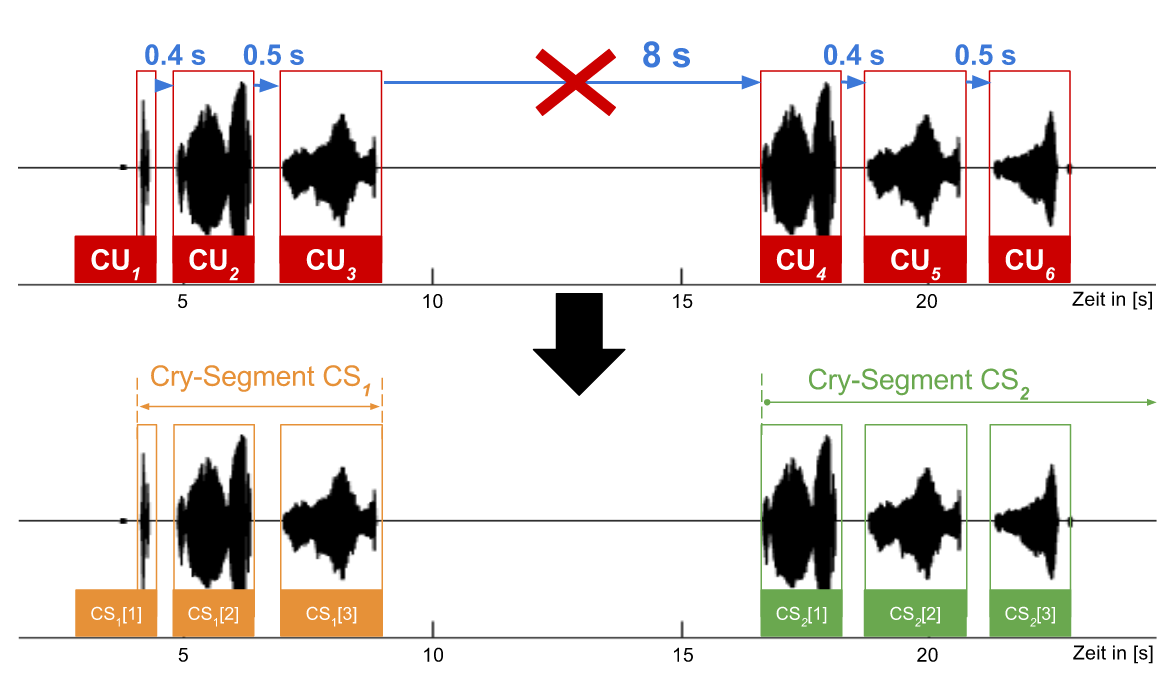
\includegraphics[width=0.75\textwidth]{bilder/segmentierung06.png}
	\caption{Ergebnis der Segmentierung}
	\label{img:segmenting03}
\end{figure}


Die Zusammenfassung von Cry-Units zu Cry-Segmentes unterliegt einer gewissen subjektiven Einschätzung, welche Cry-Units als Zuammengehörig angesehen werden, insbesondere, wenn kein erkennbarer Stimulus vorliegt. Abbildung \ref{img:segmenting02} verdeutlicht das Problem. 

\begin{figure}[H]
	\centering
	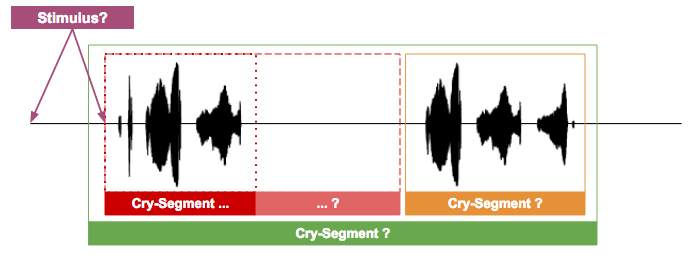
\includegraphics[width=0.48\textwidth]{bilder/segmentierung04.png}
	\caption{Mögliche Segmentierungen eines Signals}
	\label{img:segmenting02}
\end{figure}

Um das Problem zu objektivieren, wird es mathematisch formuliert. 
Eine \emph{Cry-Segment} $[CS]$ wird als Datentyp nach Formel \ref{eq:cry-segment} definiert. Ein Cry-Segment ist folglich eine Liste aufeinander folgenden Cry-Units, die gruppiert werden. Der Start-Zeitpunkt eines Cry-Segmentes wird nach Formel \ref{eq:cry-segment-start} als der Startzeitpunkt der ersten Cry-Unit des Segmentes definiert. Die Begründung für diese Entscheidung liegt darin, dass rein aus dem Audiomaterial der Zeitpunkt des Stimulus nicht festgestellt werden kann und das Segment mit Sicherheit erst bei der ersten feststellbaren Cry-Unit beginnt. Das Ende eines Segmentes wird definiert als das Ende der letzten Cry-Unit nach Gleichung \ref{eq:cry-segment-end}. Die Begründung liegt darin, dass das Ende der Reaktion auf den Stimulus ebenfalls rein aus dem Audiosignal abgeleitet werden kann und somit der einzig feststellbare Indikator die letzte Cry-Unit des Segmentes ist. 

\begin{equation}
CS = [cu_1 ,  ... ,  CU_n]
\label{eq:cry-segment}
\end{equation}

\begin{equation}
start(CS) = CS[1].start
\label{eq:cry-segment-start}
\end{equation}

\begin{equation}
end(CS) = CS[end].end
\label{eq:cry-segment-end}
\end{equation}

Wurde bei der kontinuierlichen Analyse des Signals ein Segment geschlossen, führt die Markierung einer neuen Cry-Unit zur Eröffnung eines neuen Segmentes, dessen Start-Zeitpunkt der Start-Punkt dieser Cry-Unit ist. Die Frage ist, welches Kriterium zum schließen dieses Segments führt. Laut Golub et al \cite{cryModel} ein Cry-Segment \glqq die komplette klangliche Antwort auf einen spezifischen Stimulus \grqq. Eine mögliche und objektiv messbare Interepration dieses Endes ist, dass nach dem Auftreten von Cry-Units eine längere Stille mit einer  Abwesenheit von Cry-Units festgestellt wird, da das Baby \glqq aufgehört hat, zu weinen \grqq. Übertragen auf die in \ref{sec:CryUnit} vorgestellte Terminologie heißt das, dass ein Segment beendet und ein neues begonnen wird, wenn die Distanz (Zeitraum der Stille) zwischen zwei benachbarten Cry-Units d$(CU_{i}, CU_{i+1})$ einen gewissen Grenzwert $t_{seg-max}$ überschreitet. Gleichung \ref{eq:cry-segment-constraint1} formalisiert diesen Zusammenhang. Daraus lässt sich schlussfolgern, dass die Distanzen zwischen allen benachbarten Cry-Unit eines Segmentes unter diesem Grenzwert $t_{seg-max}$ liegen. Gleichung \ref{eq:cry-segment-constraint2} formalisiert diese Nebenbedingung an die Cry-Units eines Segmentes. 

\begin{equation}
d(cu_i, cu_{i+1}) > t_{seg-max} \rightarrow CS_{n} =[CS_n, cu_i] \wedge CS_{n+1} = [cu_{i+1}]  
\label{eq:cry-segment-constraint1}
\end{equation}

\begin{equation}
\forall i = 1 ... \text{length}(CS)-1: \text{d}(CS[i], CS[i+1]) \leq t_{seg-max}
\label{eq:cry-segment-constraint2}
\end{equation}

Die einfachste Art, $t_{seg-max}$ festzulegen, ist, einen festen Grenzwert von $t$ s zuzuweisen. Abbildung \ref{img:segmenting03} visualisiert die so resultierende Segmentierung an einem Beispiel. Jeder Grenzwert mit $t_{seg-max} > \SI{0.5}{\second}$ würde zu der gezeigten Segmentierung führen. 

Algorithmus \ref{alg:crySegment} zeigt die Segmentierung nach diesem Prinzip in Pseudo-Code. Input des Algorithmus ist die Liste aller Cry-Units $CU_{all} = [cu_1 ... cu_n]$, die nach dem Decision-Smoothing nach Algorithmus \ref{alg:decisionSmoothing} entstanden ist.  Das Ergebnis des Algorithmus ist die Liste, die alle gefundene Cry-Segmente  $[cs_1 ...  cs_n]$ enthält. 

\begin{algorithm}[H]
	\caption{Gruppierung von Cry-Units zu Cry-Segments}
	\label{alg:crySegment}
	\begin{algorithmic}[1]
		\Function{segmentCryUnits}{$CU_{all}, t_{seg-max}$}
		\State $ CS_{all} \gets []$
		\State $ cs_i \gets [CU_{all}[1]]$
		\For{ $i = 2...length(CU_{all})$}
		\State $ cu_i \gets CU_{all}[i]$
		\State $cu_{i-1} \gets CU_{all}[i-1]$
		\If{d$(cu_{i-1},cu_i) < t_{seg-max}$}
		\State $cs_i \gets [cs_i , cu_i]$
		\Else
		\State $CS_{all} \gets [CS_{all}, cs_i]$
		\State $cs_i \gets [cu_i]$
		\EndIf
		\EndFor
		\Return $CS_{all}$
		
		\EndFunction
		
	\end{algorithmic}
\end{algorithm}

Algorithmus  \ref{alg:crySegment} kann zwar kontinuierlich durchgeführt werden, da er jeweils nur auf die aktuelle gefundene und eine vergangene Cry-Unit zurückgreift, hat in dieser Form jedoch den nachteil, dass das Ende eines Segmentes später als notwendig festgestellt wird. Angenommen, ein Grenzwert von $t_{seg-max} = \SI{20}{\second}$ wurde festgelegt


Bei einer kontinuierlichen durchgeführten Segmentierung wird das erste Segment dann eröffnet, sobald die erste Cry-Unit durch die VAD markiert wurde, und diese Cry-Unit dem Segment hinzugefügt. Die Dauer der Stille nach dieser Cry-Unit wird kontinuierlich gemessen. Wird ein nächste Cry-Unit festgestellt, bevor die Stille $d_{seg-max}$ übersteigt, so wird diese Cry-Unit dem Segment hinzugefügt und das Messen der Stille nach dieser Cry-Unit beginnt von vorne. Dieser Prozess wird so lange wiederholt, bis die Dauer der Stille nach einer hinzugefügten Cry-Unit $d_{seg-max}$ übersteigt. Dann wird das Segment beendet und der Endzeitpunt des Segmentes auf den Endzeitpunkt der letzten Cry-Unit gesetzt. Abbildung \ref{img:segmenting03} zeigt die resultiderende Segmentierung für Beispielsignal mit $d_{seg-max}  = \SI{3}{\second}$. Tatsächlich würde in dem Beispiel jeder Grenzwert $d_{seg-max} >\SI{0.5}{\second}$ zur gezeigten Segmentierung führen.

Es gibt verschiedene Möglichkeiten, die höchst mögliche Pause d$_{seg-max}$ zu definieren. Der Einfachste Fall, der auch in Abbildung \ref{img:segmenting03} angenommen wurde, ist das Setzen eines global festlegten Grenzwertes. Weitere Möglichkeiten sind, d$_{seg-max}(CS)$ als Funktion des Segmentes selber zu gestalten. So könnte beispielsweise ein längeres Segment eine höhere maximal-Pause erzeugen. 

Schlussendlich konnten in der Fachliteratur keine konkreten Hinweise zur Bestimmung von d$_{seg-max}$ gefunden werden. Daher wurde entschieden, dem Arzt, der das System benutzt, selber einstellen zu lassen. Es wird mit einem Festen 

\section{Feature-Extraction}
\section{Ableitung der Schmerz-Scores}
\section{Visualisierung}